
\documentclass{article}
\usepackage{graphicx}
\graphicspath{ {pictures/} }
\begin{document}

\title{Routing a robot to collect data from $n$ underwater sensors in minimum time}
\author{Srikanth K.V.S., Aaron T.\ Becker}
\maketitle

\begin{figure}[htb]
\begin{center}
	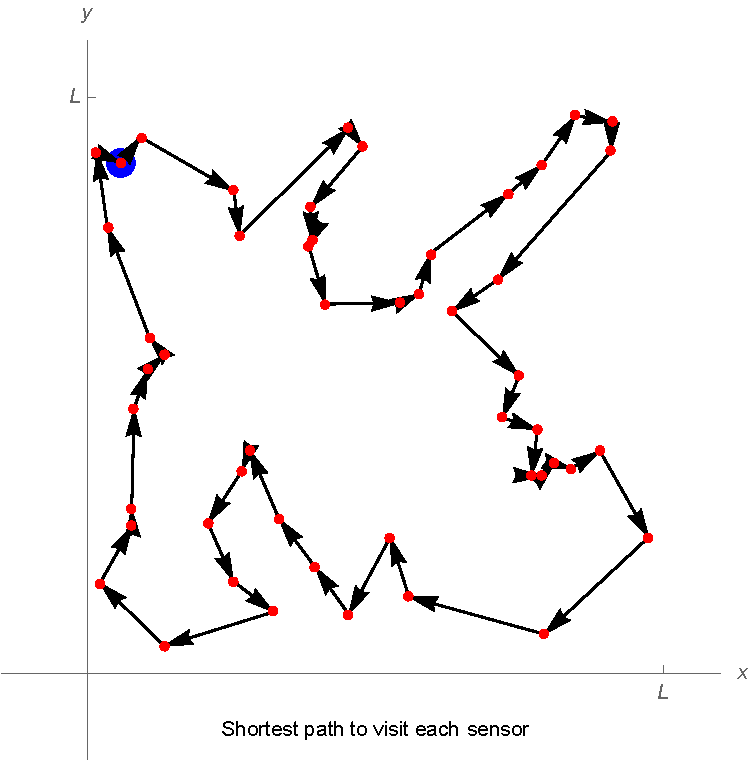
\includegraphics[width=0.48\columnwidth]{ShortestPathToSensors}
	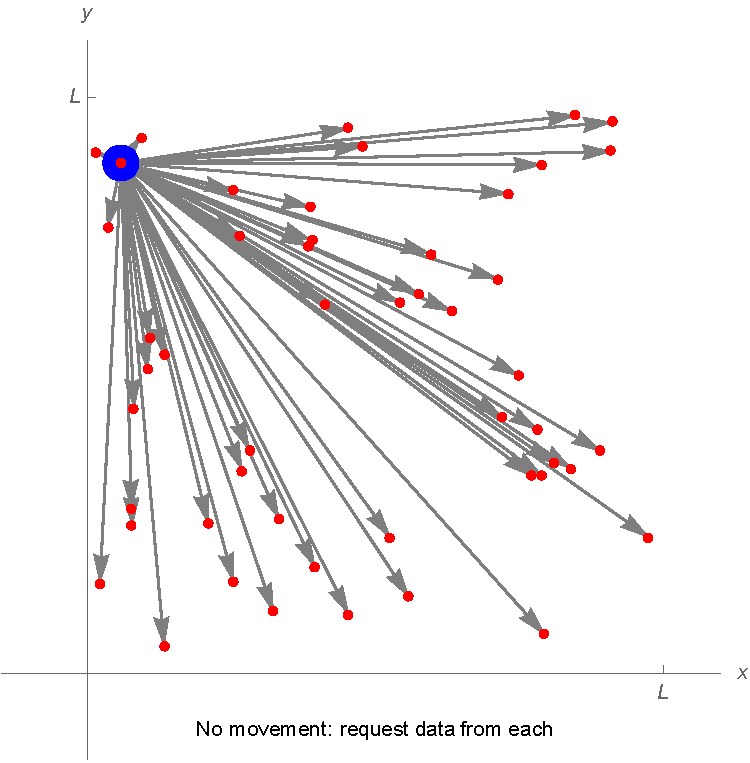
\includegraphics[width=0.48\columnwidth]{CommToEachSensor}
\end{center}
\caption{Data from $n$ nodes can be acquired by visiting each node, or by staying in place and communicating to each node.
\label{fig:ShortestPath}}
\end{figure}




\section{Introduction}

 Assume $n$ underwater sensor nodes must transmit data to a mobile underwater robot located at a depot.  We wish to minimize the total time required to transmit this data. 
The robot could potentially shorten transmission time by moving towards nodes to increase data transmission rate.
We assign $N$ waypoints on the two dimensional plane whose positions decide the path of the robot. The robot travels along the straight line joining two waypoints. The routing problem implies the robot travels in interesting closed paths to accomplish the task of collecting data hence has to traverse $N+1$ waypoints to complete a closed path. the waypoint $N = 0$ will act as a depot for offloading the collected data and recharging.
This paper examines the motion planning problem for a mobile robot to collect data from all nodes in the minimum time.  

\section{Time for servicing $n$ sensor nodes (Moving)}
\begin{figure}[htb]
\begin{center}
	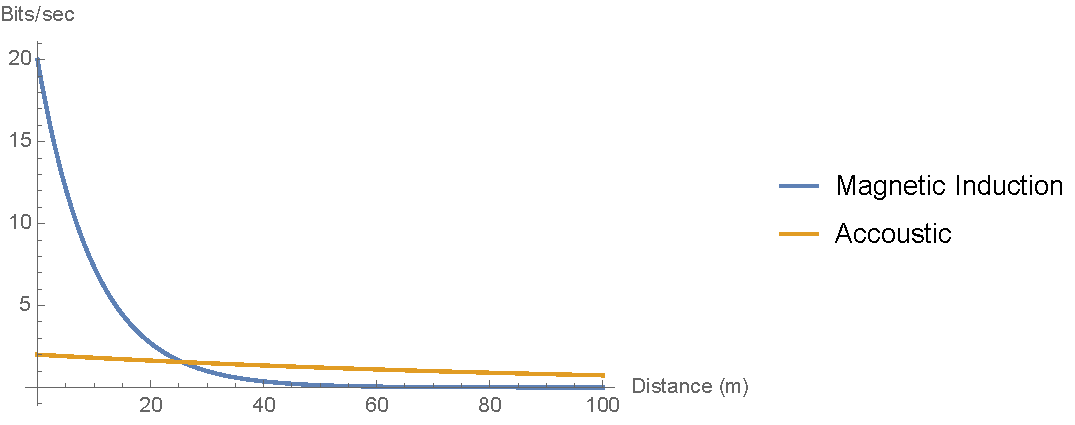
\includegraphics[width=0.48\columnwidth]{CommModel}
	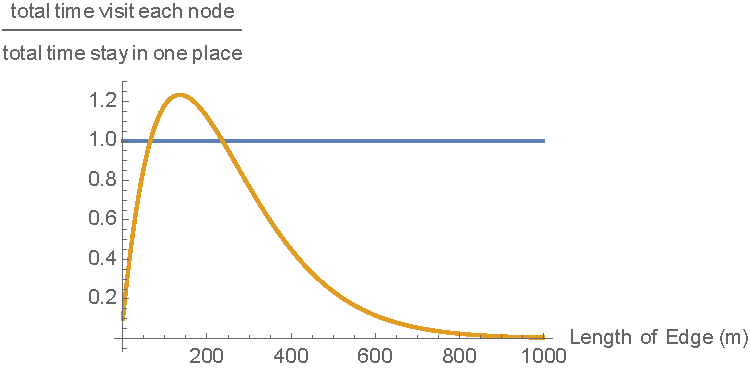
\includegraphics[width=0.48\columnwidth]{CompareVisitEachToComm}
\end{center}
\caption{Two communications models, each based on exponential decay. The two techniques shown in Fig.\ \ref{fig:ShortestPath} have differing costs as a function of the length of the workspace edges.
\label{fig:CommModel}}
\end{figure}
 Data Collection can be performed by either Magnetic Induction or Acoustic. Both methods have their advantages and disadvantages. Thus we combine both to improve efficiency.
\\
\begin{center}
\begin{tabular}{ c c }
 Data Rate for Magnetic Induction & $= D.R_{MI}$ \\ 
 Data Rate for Acoustic  & $= D.R_{Ac}$ \\  
 Velocity of the robot & $= v$  \\ 
 Data stored in each sensor node   & $= Data(j)$\\
\end{tabular}
\end{center}

\begin{equation}
    \label{TimeEqn_Moving}
   Time_{\textrm{visit each node}}  = [1/v \sum_{i=0}^{n+1} \|W_{p}(i)-W_{p}(i-1)\|] + [1/D.R. \sum_{j=1}^{n} Data(j)]    
\end{equation}
The first term in equation 1 indicates\textbf{ travel time}.\\*
The second term indicates the \textbf{transmission time}.\\*
For obtaining the solution we will use a TSP (Traveling Salesman Problem) solver.

\section{Time for servicing $n$ sensor nodes (Stationary)}

\begin{equation}
    \label{TimeEqn_Stationary}
    Time_{\textrm{stay at depot}} = 0 + \sum_{i=1}^{n} \|P_{i}-P_{o}\| 
    \end{equation} 
\begin{equation}
    \label{Transmission}
    min_{(1/D.R_{MI})}*(Dist),min_{(1/D.R_{Ac})}*(Dist)  
\end{equation}
0 refers to the the traveling cost.\\*
The rest is the transmission cost.

\section{General Cost}
\label{GeneralCost_SingleMode}
\begin{equation}
1/v \sum_{i=0}^{n+1} \|W_{p}(i)-W_{p}(i-1)\|+\sum_{i=0}^{n+1}\sum_{j=1}^{n} a_{ij}*Min ((1/D.R)*\|W_{p}(i)-P{j}\|)
\end{equation}
Constraints:
\label{GeneralCostSingle_Constraints}
\begin{equation}
\sum_{i=0}^{n+1} a_{ij} = Data_{j}, \forall j \in [1,n], 
 a_{ij}\geq 0
\end{equation}

\label{Dist_Definition}
\begin{equation}
D = \|W_{p}(i)-P{j}\|
\end{equation}

\label{GeneralCost_DoubleMode}
\begin{equation}
1/v \sum_{i=0}^{n+1} \|W_{p}(i)-W_{p}(i-1)\|+\sum_{i=0}^{n+1}Max(\sum_{j=1}^{n} \times a_{ij}\times D/D.R_{MI}(Dist))  
\end{equation}
\begin{equation}
(\sum_{j=1}^{n} b_{ij}\times D/D.R_{Ac}(Dist))
\end{equation}

Constraints:
\label{GeneralCostDouble_Constraints}
\begin{equation}
\sum_{i=1}^{n+1} a_{ij}+b_{ij}=Data,\forall i \in [1,n], 
 a_{ij}\geq 0,b_{ij}\geq 0
\end{equation}
\end{document}